\documentclass[a4paper]{article}

%\usepackage[ngerman]{babel}
\usepackage[T1]{fontenc}
\usepackage[utf8]{inputenc}
\usepackage{textcomp}
\date{}
\author{}
\usepackage{geometry}
\geometry{ left=2cm, right=2cm, top=2cm, bottom=4cm, bindingoffset=5mm}

\usepackage{graphicx}
\usepackage{xcolor}
\usepackage{hyperref}
\usepackage{fancyhdr}
\pagestyle{fancy}
\fancyhf{}
\fancyhead[R]{2973140 - Felix Bühler  \\ 2893121 - Jan Leusmann \\  3141241 - Jamie Ullerich}
\fancyhead[L]{Scientific Visualisation \\ Sommersemester 2019 }
\renewcommand{\headrulewidth}{0.5pt}

\title{Exercise 3}

\begin{document}
	
	\maketitle
	\thispagestyle{fancy}
	
	\section*{Exercise 3.1 - Cartesian Grids}
	% vis 03 Folie 41
	% https://stackoverflow.com/questions/29142417/4d-position-from-1d-index
	$I[i, j, k, l] = l\cdot K \cdot M \cdot N  + k \cdot M \cdot N  + j \cdot N + i$
	
	\section*{Exercise 3.2 - ParaView Introduction: Point Splatting}
	
	\begin{figure}[!ht]
		\centering
		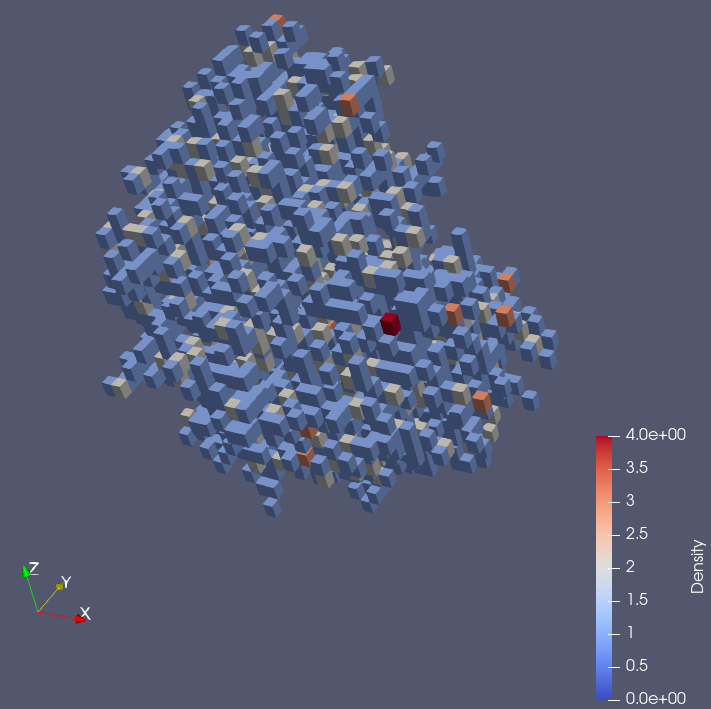
\includegraphics[width=0.7\linewidth]{paraview}
		\caption{Correct - Output}
		\label{fig:paraview}
	\end{figure}
	
	
	
\end{document}
